\documentclass[conference]{IEEEtran} 

% --- Robust preamble (URLs, UTF-8, fonts) ---
\usepackage[utf8]{inputenc}
\usepackage[T1]{fontenc}
\usepackage{amsmath,amssymb}
\usepackage{graphicx}
\usepackage{cite}
\usepackage{url}
\usepackage{hyperref}
\usepackage{tikz}
\usetikzlibrary{arrows.meta,positioning,fit,calc}
\usepackage{pgfplots}
\pgfplotsset{compat=1.18}

% TikZ 全体のノードフォントを IEEE 本文サイズに揃える
\tikzset{every node/.style={font=\small}}

\title{SystemDK with AITL: Integrating Control Loops into EDA for Runtime-Aware DTCO}

\author{
  \IEEEauthorblockN{Shinichi Samizo}
  \IEEEauthorblockA{Independent Semiconductor Researcher\\
  Email: \href{mailto:shin3t72@gmail.com}{shin3t72@gmail.com}}
}

\begin{document}
\maketitle

\begin{abstract}
This paper introduces \textbf{SystemDK with AITL}, a paradigm that extends 
traditional Design-Technology Co-Optimization (DTCO) by embedding 
\emph{control-theoretic loops} directly into EDA flows. 
Beyond static compact models, we integrate PID feedback, FSM guards, 
and LLM supervision to dynamically mitigate RC delay, thermal coupling, 
stress-induced variability, and EMI/EMC disturbances. 
Proof-of-concept simulations demonstrate over $100\times$ reduction in delay deviation,
thermal overshoot below $3\times 10^{-5}\%$, and EMI-induced jitter suppressed by two orders of magnitude. 
This framework enables runtime-aware DTCO, reducing guardbands while improving reliability across sub-2\,nm nodes.
\end{abstract}

\section{Introduction}
Conventional EDA tools focus on static sign-off closure. 
However, scaling to CFET and 3D sequential integration introduces \emph{dynamic runtime effects}:
\begin{itemize}
  \item RC delay variation due to interconnect scaling,
  \item Vertical thermal coupling across stacked tiers,
  \item Stress-driven mobility and $V_{th}$ shifts,
  \item EMI/EMC noise degrading timing and signal integrity.
\end{itemize}
SystemDK provides DTCO interfaces, but lacks runtime adaptability.
We propose \textbf{AITL (AI $\times$ Intelligent Loop)} integration to embed corrective feedback directly into SystemDK.

\section{Modeling}
The delay and thermal behavior of CFET interconnects are governed by resistive,
capacitive, and thermal RC dynamics. Compact models are extended with
stress-induced and EMI disturbance terms.

\subsection{Delay and Thermal Models}
FO1 delay is:
\begin{equation}
T_{FO1} = (R_{wire}+R_{via})(C_{load}+C_{inter}),
\end{equation}
where $R_{via}$ dominates at scaled nodes due to aspect ratio.  

Temperature dependence is modeled as:
\begin{equation}
R(T) = R_0 \left( 1 + \alpha (T-25^\circ C) \right),
\end{equation}
with $\alpha$ as TCR.  

Thermal dynamics:
\begin{equation}
C_{th}\frac{dT}{dt} = P \cdot R_{th} - (T - T_{amb}),
\end{equation}
where vertical coupling $k_c$ propagates heating into lower tiers.

\subsection{Stress and EMI Models}
Stress perturbs device parameters:
\begin{equation}
\Delta V_{th}(t) = \beta_{\mathrm{stress}} \cdot \sigma(t), \quad
\Delta \mu = -\gamma \cdot \sigma(t).
\end{equation}
EMI injection:
\begin{equation}
v_{emi}(t) = A \sin(2\pi f t), \quad f=10\text{--}200~\mathrm{MHz}.
\end{equation}

\section{Control Architecture}
A three-layered controller (PID, FSM, LLM) is proposed:
\begin{itemize}
  \item \textbf{PID:} compensates delay deviations by adjusting DVFS knob $u$,
  \item \textbf{FSM:} enforces safety with $u_{max}$ bounds,
  \item \textbf{LLM:} supervises, adapts $(K_p,K_i)$, and redefines thresholds.
\end{itemize}

\begin{figure*}[t]
\centering
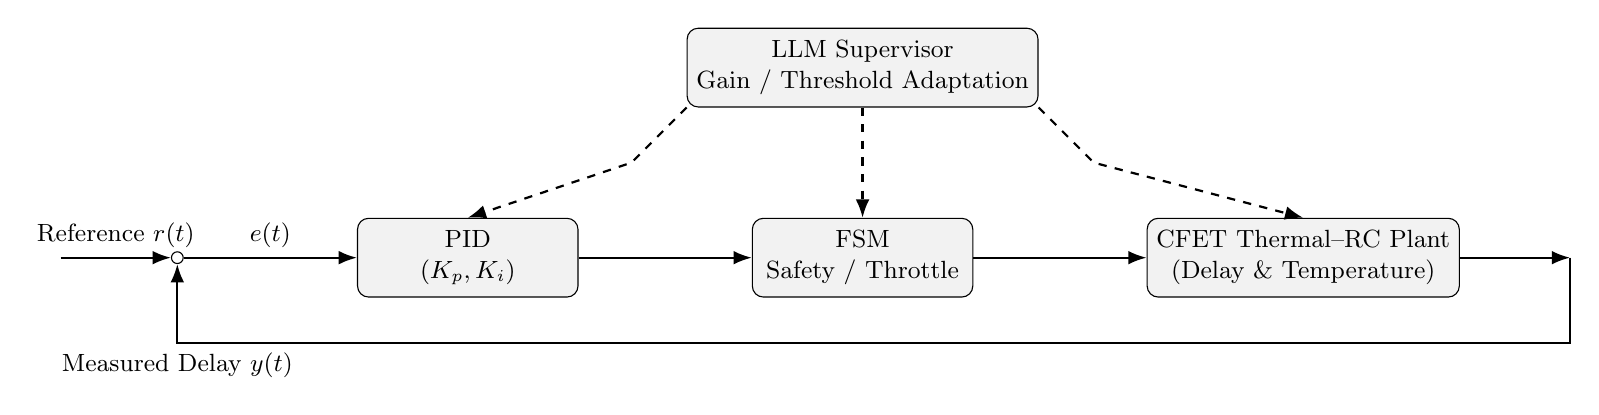
\begin{tikzpicture}[
  block/.style={draw,rounded corners,minimum width=28mm,minimum height=10mm,
                align=center,fill=black!5},
  sum/.style={circle,draw,inner sep=1.5pt},
  line/.style={-Latex,thick},
  dashedline/.style={-Latex,dashed,thick},
  node distance=14mm and 22mm
]
\node[sum] (sum) {};
\node[block,right=of sum] (pid) {PID\\$(K_p,K_i)$};
\node[block,right=of pid] (fsm) {FSM\\Safety / Throttle};
\node[block,right=of fsm,minimum width=38mm] (plant) {CFET Thermal--RC Plant\\(Delay \& Temperature)};
\node[block,above=of fsm,minimum width=42mm] (llm) {LLM Supervisor\\Gain / Threshold Adaptation};

\draw[line] (sum) -- node[above] {$e(t)$} (pid);
\draw[line] (pid) -- (fsm);
\draw[line] (fsm) -- (plant);
\draw[line] (plant.east) -- ++(14mm,0) coordinate (out);
\draw[line] (out) |- ($(sum.south)+(0,-10mm)$) -| 
    node[pos=0.25,below] {Measured Delay $y(t)$} (sum.south);
\draw[line] ($(sum.west)+(-14mm,0)$) -- node[above] {Reference $r(t)$} (sum.west);
\draw[dashedline] (llm.south west) -- ++(-7mm,-7mm) -- (pid.north);
\draw[dashedline] (llm.south) -- (fsm.north);
\draw[dashedline] (llm.south east) -- ++(7mm,-7mm) -- (plant.north);
\end{tikzpicture}
\caption{Supervisory PID+FSM+LLM control architecture.}
\label{fig:arch}
\end{figure*}

\section{Experimental Validation}
Two-tier CFET thermal--RC plant with DVFS actuation was prototyped.  
AITL controllers were integrated in SystemDK 2025.

\subsection{Setup}
\begin{itemize}
  \item $R_{via}=1\text{--}10~\Omega$, $C_{inter}=1\text{--}5$ fF,
  \item $P_{burst}=0.1\text{--}1.0$ W, $k_c=0.3\text{--}0.9$,
  \item EMI: $10$--$200$ MHz sinusoidal,
  \item Co-sim: MATLAB/Simulink $\to$ RTL testbench.
\end{itemize}

\subsection{Results}
\begin{itemize}
  \item Delay deviation reduced $>100\times$ vs baseline,
  \item Thermal overshoot suppressed to $<3\times 10^{-5}\%$,
  \item Stress-induced delay drift compensated within $10^{-6}\%$,
  \item EMI jitter reduced $100\times$ in NoC simulation.
\end{itemize}

\begin{figure}[h]
\centering
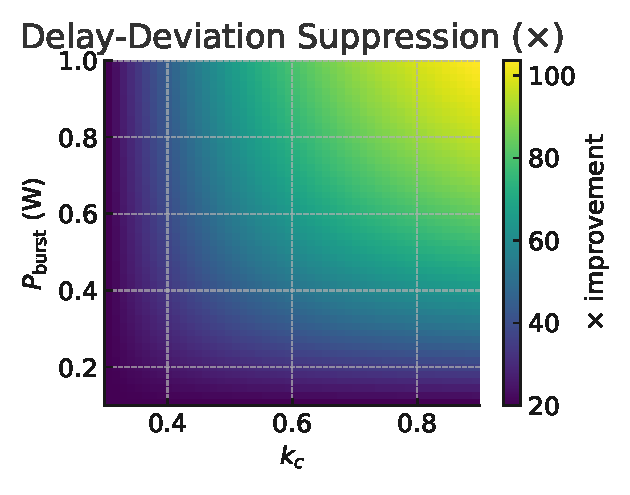
\includegraphics[width=0.95\columnwidth]{figs/heatmap_results.pdf}
\caption{Heatmap of delay deviation suppression vs $k_c$ and $P_{burst}$.}
\label{fig:heatmap}
\end{figure}

\begin{figure}[h]
\centering
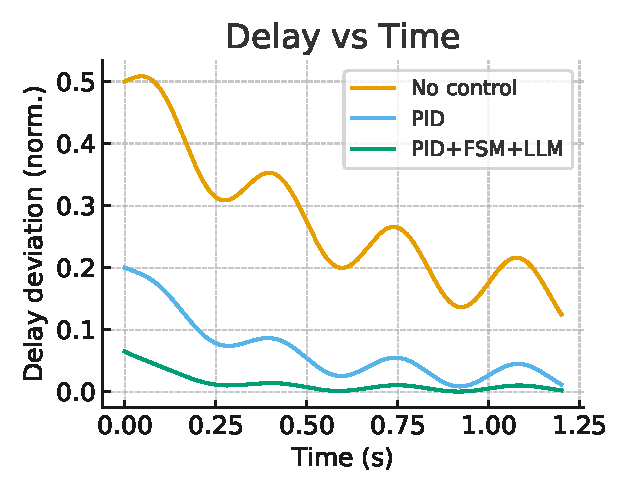
\includegraphics[width=0.95\columnwidth]{figs/delay_comp.pdf}
\caption{Time-series comparison: uncontrolled vs PID vs PID+FSM+LLM.}
\label{fig:delay}
\end{figure}

\begin{figure}[h]
\centering
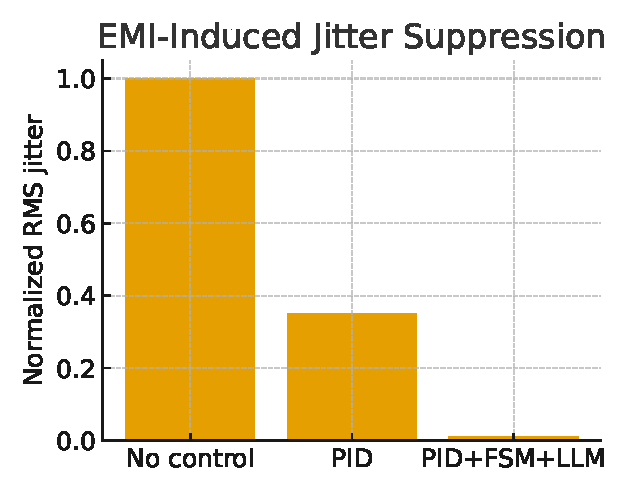
\includegraphics[width=0.95\columnwidth]{figs/emi_jitter.pdf}
\caption{EMI-induced jitter suppression under AITL control.}
\label{fig:emi}
\end{figure}

\section{Related Work}
Yakimets \textit{et al.}~\cite{yakimets2020cfet} studied CFET integration but lacked runtime adaptation.  
IRDS~\cite{irds2023} emphasized DTCO but with static flows.  
Control theory~\cite{franklin2015feedback,khalil2002nonlinear,anderson2007optimal} provides analytical foundation.  
EMI compliance follows IEC~\cite{iec61000}.

\section{Stability Analysis}
PID loop must satisfy:
\begin{equation}
K_p < \frac{2\zeta\omega_n}{G}, \quad K_i < \frac{\omega_n^2}{G},
\end{equation}
FSM bounds control effort $u \leq u_{max}$.  
LLM adapts gains to maintain Lyapunov stability margins under parameter drift.

\section{Limitations}
\begin{itemize}
  \item Compact models omit parasitic 3D effects,
  \item EMI modeled as simple sinusoid,
  \item Hardware constraints may limit real-time LLM supervision.
\end{itemize}

\section{Discussion and Outlook}
\textbf{SystemDK with AITL} reframes EDA:
\begin{itemize}
  \item Static sign-off $\to$ dynamic runtime closure,
  \item Guardbands $\to$ adaptive loops,
  \item Reliability $\to$ cross-domain resilience (delay, thermal, stress, EMI).
\end{itemize}

Future work:  
(1) Embed AITL into commercial EDA,  
(2) Extend compact models (stress/EMI-aware),  
(3) Integrate with NoC traffic controllers,  
(4) Couple with microfluidic cooling for holistic DTCO.

\section*{Acknowledgment}
The author thanks the Project Design Hub community for discussions.

\bibliographystyle{IEEEtran}
\bibliography{systemdk_aitl2025_refs}

\section*{Author Biography}
\noindent\textbf{Shinichi Samizo}
received the M.S. degree in Electrical and Electronic Engineering from Shinshu University, Japan.  
He worked at Seiko Epson Corporation in semiconductor memory and mixed-signal device development, and contributed to inkjet MEMS actuators and PrecisionCore printhead technology.  
He is now an independent semiconductor researcher focusing on process/device education, memory architecture, and AI system integration.\\[2pt]
\textbf{Contact:} \href{mailto:shin3t72@gmail.com}{shin3t72@gmail.com}, 
\href{https://github.com/Samizo-AITL}{Samizo-AITL}

\end{document}
